% v2/main.tex — PhD dissertation entry point.
%
% Document format is unchanged from v1 (RIT GCCIS one-column book class +
% thesisfrontmatter). What is new in v2 is the build system, borrowed from
% the onlycodes paper (hyang0129/onlycodes/paper):
%
%   * Every number in prose resolves at build time through \result-family
%     macros (macros.tex), backed by data/*.csv via build_numbers.py.
%   * `make lint` (lint.py) is the BIB GATE: it fails the build on any bare
%     digit in prose that is not inside a \result{}/\cite{}/\ref{} macro,
%     a year, or a whitelisted string. A stale number is a build failure,
%     not a proofreading task.
%   * references.bib is human-gated — agents propose citations in outlines/
%     first; the .bib is never edited by an agent directly.
%
% Build with:  make paper   (see README.md / Makefile)

\documentclass[11pt, oneside]{book}

\usepackage[phd]{thesisfrontmatter}
%\usepackage[proposal]{thesisfrontmatter}  % uncomment for the proposal variant

\input{math_commands.tex}

\newcommand{\cX}{\mathcal{X}}
\newcommand{\cD}{\mathcal{D}}

\setlength{\parindent}{0pt}

% --- Math / tables / figures -------------------------------------------------
\usepackage{amsmath}
\usepackage{amssymb}
\usepackage{amsfonts}
\usepackage{mathtools}
\usepackage{amsthm}
\usepackage{booktabs}
\usepackage{multicol}
\usepackage{graphicx}
\usepackage{subfigure}
\usepackage{wrapfig}
\usepackage{xcolor}
\usepackage{colortbl}
\usepackage{placeins}
\usepackage{tikz}
\usetikzlibrary{positioning,shapes,arrows,calc,fit}
\usepackage{algorithm}
\usepackage{algpseudocode}
\usepackage[hyphens]{url}
\usepackage[toc,page]{appendix}
\usepackage{geometry}

% --- Bibliography (natbib; references.bib is human-gated) --------------------
\usepackage{natbib}

% --- Theorem environments (the dissertation carries formal proofs) ----------
\theoremstyle{plain}
\newtheorem{theorem}{Theorem}[section]
\newtheorem{proposition}[theorem]{Proposition}
\newtheorem{lemma}[theorem]{Lemma}
\newtheorem{corollary}[theorem]{Corollary}
\theoremstyle{definition}
\newtheorem{definition}[theorem]{Definition}
\newtheorem{assumption}[theorem]{Assumption}
\newtheorem{method}[theorem]{Method}
\theoremstyle{remark}
\newtheorem{remark}[theorem]{Remark}

% --- BIB GATE infrastructure -------------------------------------------------
% \result, \resdelta, \resratio, \resultCI, \resultPM, ... (single source of
% truth for every number). values.tex is generated by build_numbers.py; if
% absent (drafting before a build), the \IfFileExists guard lets the document
% still compile and macros render as ?? until `make values` is run.
% macros.tex
% Late-binding citation macros for the dissertation paper.
%
% Every number in prose resolves at build time through these macros.
% Values are defined in generated/values.tex via \csname lookup;
% build_numbers.py produces that file from data/*.csv and
% generated/figures/*.numbers.csv.
%
% Namespace prefix: ds@ (dissertation). Must match NAMESPACE in build_numbers.py.
%
% Usage:
%   \result{csv_stem}{key}[precision]
%   \resdelta{csv_stem}{key_a}{key_b}[precision]
%   \resratio{csv_stem}{key_a}{key_b}[precision]
%   \resultCI{csv_stem}{mean_key,lo_key,hi_key}[precision]
%   \resultPM{csv_stem}{mean_key,err_key}[precision]
%
% Where:
%   csv_stem  - stem of the CSV file (e.g. "headline" for headline.csv,
%               "fig.02_signflip" for the sidecar of Figure 2 — note the
%               filename is still 02_signflip.* for build-pipeline stability
%               even though the §5.3 prose framing was retuned 2026-05-28;
%               see paper/05_results.md §5.3 for the rationale)
%   key       - colon-joined coordinate per the CSV's key_schema
%   precision - number of decimal places for siunitx rounding (optional;
%               default is the CSV's default_precision, embedded as
%               ds@<stem>@__default_precision__ in values.tex)

\usepackage{siunitx}
\usepackage{xfp}
\usepackage{etoolbox}

% --------------------------------------------------------------------------
% Definitions below use @ in macro names. Outside a .sty file, @ has catcode
% 12, so we temporarily make it a letter via \makeatletter / \makeatother.
% --------------------------------------------------------------------------
\makeatletter

% --------------------------------------------------------------------------
% Internal helper: look up \csname ds@<stem>@<key>\endcsname
% Raises \PackageError if undefined.
% --------------------------------------------------------------------------
\newcommand{\ocget}[2]{%
  \@ifundefined{ds@#1@#2}{%
    \PackageError{dissertation-macros}%
      {Undefined result key '#2' in CSV stem '#1'.
       Check data/#1.csv and re-run 'make values'.}%
      {The key '#2' was not found in the values generated from '#1'.
       Valid keys are listed in generated/values.tex.}%
    \textbf{??}%
  }{%
    \csname ds@#1@#2\endcsname%
  }%
}

% --------------------------------------------------------------------------
% Helper: get default precision for a CSV stem (falls back to 3)
% --------------------------------------------------------------------------
\newcommand{\ocgetdefprec}[1]{%
  \@ifundefined{ds@#1@__default_precision__}{3}{\csname ds@#1@__default_precision__\endcsname}%
}

% --------------------------------------------------------------------------
% \result{csv}{key}[precision]
% --------------------------------------------------------------------------
\DeclareRobustCommand{\result}[2]{%
  \@ifnextchar[%]
    {\ds@result@prec{#1}{#2}}%
    {\ds@result@prec{#1}{#2}[\ocgetdefprec{#1}]}%
}
\def\ds@result@prec#1#2[#3]{%
  \num[round-mode=places,round-precision=#3]{\ocget{#1}{#2}}%
}

% --------------------------------------------------------------------------
% \resdollar{csv}{key}[precision]
% Render a USD value with the sign OUTSIDE the dollar sign: a negative
% value prints as "-\$0.023", not "\$-0.023". Rounds first so that values
% that round to zero print "\$0.000" rather than "-\$0.000". Use inside
% math mode (the bare "-" is a math minus), mirroring the old
% "$\$\result{...}$" idiom that placed the minus after the dollar sign.
% --------------------------------------------------------------------------
\DeclareRobustCommand{\resdollar}[2]{%
  \@ifnextchar[%]
    {\ds@dollar@prec{#1}{#2}}%
    {\ds@dollar@prec{#1}{#2}[\ocgetdefprec{#1}]}%
}
\def\ds@dollar@prec#1#2[#3]{%
  \edef\ds@dv{\fpeval{round(\ocget{#1}{#2},#3)}}%
  \ifnum\fpeval{\ds@dv<0}=1 %
    -\$\num[round-mode=places,round-precision=#3]{\fpeval{abs(\ds@dv)}}%
  \else
    \$\num[round-mode=places,round-precision=#3]{\ds@dv}%
  \fi
}

% --------------------------------------------------------------------------
% \resdelta{csv}{key_a}{key_b}[precision]
% Computes key_a - key_b using \fpeval from xfp.
% (Named \resdelta, not \delta, to avoid clashing with the Greek letter.)
% --------------------------------------------------------------------------
\DeclareRobustCommand{\resdelta}[3]{%
  \@ifnextchar[%]
    {\ds@delta@prec{#1}{#2}{#3}}%
    {\ds@delta@prec{#1}{#2}{#3}[\ocgetdefprec{#1}]}%
}
\def\ds@delta@prec#1#2#3[#4]{%
  \edef\ds@va{\ocget{#1}{#2}}%
  \edef\ds@vb{\ocget{#1}{#3}}%
  \num[round-mode=places,round-precision=#4,explicit-sign]{\fpeval{\ds@va - \ds@vb}}%
}

% --------------------------------------------------------------------------
% \resratio{csv}{key_a}{key_b}[precision]
% Computes key_a / key_b using \fpeval.
% --------------------------------------------------------------------------
\DeclareRobustCommand{\resratio}[3]{%
  \@ifnextchar[%]
    {\ds@ratio@prec{#1}{#2}{#3}}%
    {\ds@ratio@prec{#1}{#2}{#3}[\ocgetdefprec{#1}]}%
}
\def\ds@ratio@prec#1#2#3[#4]{%
  \edef\ds@va{\ocget{#1}{#2}}%
  \edef\ds@vb{\ocget{#1}{#3}}%
  \num[round-mode=places,round-precision=#4]{\fpeval{\ds@va / \ds@vb}}%
}

% --------------------------------------------------------------------------
% \resp{csv}{key}[sigfigs]
% Render a p-value at N significant figures (default 2). Uses siunitx
% scientific notation automatically for small p (e.g. 2.7e-17 → 2.7×10⁻¹⁷),
% which `\result`'s round-mode=places would clobber to 0.000.
% --------------------------------------------------------------------------
\DeclareRobustCommand{\resp}[2]{%
  \@ifnextchar[%]
    {\ds@resp@prec{#1}{#2}}%
    {\ds@resp@prec{#1}{#2}[2]}%
}
\def\ds@resp@prec#1#2[#3]{%
  \num[round-mode=figures,round-precision=#3]{\ocget{#1}{#2}}%
}

% --------------------------------------------------------------------------
% \respp{csv}{key}[precision]
% Render a stored 0–1 fraction as percentage points: value × 100. Pass-rate
% deltas in paired_contrasts.csv are fractions; tables typically want pp.
% Default precision: 2 decimal places.
% --------------------------------------------------------------------------
\DeclareRobustCommand{\respp}[2]{%
  \@ifnextchar[%]
    {\ds@respp@prec{#1}{#2}}%
    {\ds@respp@prec{#1}{#2}[2]}%
}
\def\ds@respp@prec#1#2[#3]{%
  \num[round-mode=places,round-precision=#3]{\fpeval{100*\ocget{#1}{#2}}}%
}

% --------------------------------------------------------------------------
% \respct{csv}{delta_key}{ref_key}[precision]
% Render a paired-contrast delta as a percentage of a reference mean:
% (delta / ref) × 100, with a literal '%' appended. For "code-only is X%
% cheaper than competitor" framing, pass the contrast's mean_b cell as ref.
% Default precision: 1 decimal place.
% --------------------------------------------------------------------------
\DeclareRobustCommand{\respct}[3]{%
  \@ifnextchar[%]
    {\ds@respct@prec{#1}{#2}{#3}}%
    {\ds@respct@prec{#1}{#2}{#3}[1]}%
}
\def\ds@respct@prec#1#2#3[#4]{%
  \edef\ds@vd{\ocget{#1}{#2}}%
  \edef\ds@vr{\ocget{#1}{#3}}%
  \num[round-mode=places,round-precision=#4]{\fpeval{100*\ds@vd/\ds@vr}}\%%
}

% --------------------------------------------------------------------------
% \resultCI{csv}{mean_key,lo_key,hi_key}[precision]
% Renders as: mean [lo, hi]
% --------------------------------------------------------------------------
\DeclareRobustCommand{\resultCI}[2]{%
  \@ifnextchar[%]
    {\ds@ci@prec{#1}{#2}}%
    {\ds@ci@prec{#1}{#2}[\ocgetdefprec{#1}]}%
}
\def\ds@ci@prec#1#2[#3]{%
  \ds@splitthree{#2}{\ds@keyA}{\ds@keyB}{\ds@keyC}%
  \num[round-mode=places,round-precision=#3]{\ocget{#1}{\ds@keyA}}%
  \ [\num[round-mode=places,round-precision=#3]{\ocget{#1}{\ds@keyB}},
     \num[round-mode=places,round-precision=#3]{\ocget{#1}{\ds@keyC}}]%
}

% --------------------------------------------------------------------------
% \resultPM{csv}{mean_key,err_key}[precision]
% Renders as: mean ± err
% --------------------------------------------------------------------------
\DeclareRobustCommand{\resultPM}[2]{%
  \@ifnextchar[%]
    {\ds@pm@prec{#1}{#2}}%
    {\ds@pm@prec{#1}{#2}[\ocgetdefprec{#1}]}%
}
\def\ds@pm@prec#1#2[#3]{%
  \ds@splittwo{#2}{\ds@keyA}{\ds@keyB}%
  \num[round-mode=places,round-precision=#3]{\ocget{#1}{\ds@keyA}}%
  $\pm$%
  \num[round-mode=places,round-precision=#3]{\ocget{#1}{\ds@keyB}}%
}

% --------------------------------------------------------------------------
% Utility: split comma-delimited pairs and triples into named macros.
% --------------------------------------------------------------------------
\def\ds@splittwo#1#2#3{%
  \ds@splittwoaux#1\@nil{#2}{#3}%
}
\def\ds@splittwoaux#1,#2\@nil#3#4{%
  \def#3{#1}\def#4{#2}%
}

\def\ds@splitthree#1#2#3#4{%
  \ds@splitthreeaux#1\@nil{#2}{#3}{#4}%
}
\def\ds@splitthreeaux#1,#2,#3\@nil#4#5#6{%
  \def#4{#1}\def#5{#2}\def#6{#3}%
}

\makeatother

\IfFileExists{generated/values.tex}{\input{generated/values}}{}

\begin{document}

%*******************************************
% FRONT MATTER
%*******************************************
\pagenumbering{roman}

% frontmatter/CoverPage.tex — degree-page variables consumed by
% thesisfrontmatter.sty (\makedeclaration, \makeapproval, \abstract, ...).
% This file defines variables only; it renders nothing on its own.

\degreetitle{What Representations Preserve: Information-Theoretic and Geometric Conditions for Out-of-Distribution and Hallucination Detection}

\degreeauthor{Hong Yang}

\degreedate{[Month and Year of Dissertation Acceptance]}

%\prevdegreeA{B.S. ...}
%\prevdegreeB{M.S. ...}

\advisor{[Advisor's name]}

\memberA{[Committee member's name]}
\memberB{[Committee member's name]}
\memberC{[Committee member's name]}
\memberD{[Ph.D. Program Director name]}
\externalchair{[External Chair's name]}
   % sets \degreetitle, \degreeauthor, committee

% FOR THESIS:
\makedeclaration
\makeapproval
\makecopyright

% FOR PROPOSAL, comment the three lines above and uncomment:
%\makeproposaldeclaration
%\makePHDproposalapproval

% frontmatter/Abstract.tex — dissertation abstract.
% Plain Ch.4 register per outlines/style_guide.md. Regenerated 2026-06-09 via the
% regenerate-not-patch workflow (style_guide.md §6): re-authored from a bare-claims
% skeleton conditioned on Ch.4 rhythm spans, gated with voice_meter.py, and varied
% asymmetrically against the Ch.1 thesis statement so the shared n-grams clear.
% Must still fit ONE PAGE — keep the \linespread line; do not lengthen. Framing locks:
% representation-structure thesis, BOTH lenses; arc failure -> recovery -> detection;
% "guaranteed failure" Ch.4-only; Ch.5 diagnostic+recovery; Ch.6 = parity / "matches
% or, in the mean, outperforms", never "beats"/"superior". Bookend sentence "When the
% representation keeps it, a detector can read it out." stays verbatim (sanctioned).
\begin{abstract}
% Tighten body leading slightly so the abstract fits on one page (the global
% \linespread{1.25} pushed the final sentence onto a second page). Scoped to this
% environment's group, so it does not affect any other page.
\linespread{1.12}\selectfont
Models deployed outside controlled settings encounter inputs unlike their training
data and may generate outputs unsupported by what they learned. A reliable system
should recognize these cases. Out-of-distribution detection and hallucination
detection are usually studied separately, but both depend on the same condition:
the model's representation must retain the information that distinguishes an
anomalous case from an ordinary one. If training never captures that information,
or later suppresses it, no downstream detector can recover it.

We study this condition from two complementary perspectives. Mutual information
measures how much information about the relevant distinction remains in a
representation, while feature-space geometry shows whether the directions needed to
detect a shift retain sufficient variation. The first study proves that unlabeled
detection must fail when the self-supervised or unsupervised objective is independent
of the label-relevant features. It also introduces the Adjacent OOD benchmark to
evaluate this high-overlap regime. The second study identifies domain-sensitivity
collapse, in which single-domain training suppresses shift-sensitive directions, and
introduces Teacher-Guided Training to restore them without adding inference cost. The
third study develops a hallucination detector from cross-layer activations. Its
contrastive probe reaches parity with the strongest engineered probe and outperforms
it in the mean, consistent with the study's feasibility argument.

The unifying representation-structure framework is the central contribution. The
dissertation establishes a conditional limit on unlabeled OOD detection and
demonstrates interventions when relevant structure can be restored or read out; it
does not claim these methods are optimal.
\end{abstract}

% frontmatter/Acknowledgements.tex
\begin{acknowledgements}
I owe this work to the people who carried me to it.

To my advisor, Travis Desell, for the guidance, the patience, and the freedom to
follow the questions where they led. To my committee --- Alexander Ororbia,
Ashique KhudaBukhsh, Qi Yu, and Pengcheng Shi --- for the time, the careful
reading, and the sharper thinking their feedback demanded, and to Sharon Mason
for chairing the defense.

To my friends, who kept me steady through the long stretches and reminded me
there was a life outside the work.

And to my family, who believed in this before I did, and never once let me
doubt that I would finish.
\end{acknowledgements}

% frontmatter/Dedication.tex
\begin{dedication}
For my mother.

A single mother who worked harder than anyone I know to give me the chances she
never had. Every opportunity that led here was one she made possible. This is
hers as much as mine.
\end{dedication}


\tableofcontents
\listoffigures
\listoftables

\pagebreak
\pagenumbering{arabic}

%*******************************************
% MAIN TEXT  (one file per chapter, in chapters/)
%*******************************************
% chapters/01_introduction.tex
% Regenerated 2026-07-12 via the regenerate-not-patch workflow (style_guide.md §6).
% Sonnet 5 authored four structurally divergent drafts from a bare-claims brief
% conditioned on Ch.4 rhythm spans; the "medical-lead" draft was selected, the
% sanctioned thesis bookend placed at the opening thesis position (once), and the
% chapter gated with voice_meter.py (per-file texture + cross-chapter n-grams vs the
% neighbor framing files). Diction pass: no figurative near-miss nouns.
% Framing locks (do not violate): spine = representation structure, BOTH lenses;
% arc = failure -> recovery -> detection; "guaranteed failure" is Ch.4-only; Ch.5
% diagnostic not impossibility; Ch.6 verb "matches-or-outperforms (in the mean)" /
% parity, never "beats"/"SOTA". No results numbers. Bookend to Ch.7.
\chapter{Introduction}
\label{ch:introduction}

A model trained on chest X-rays does not necessarily hesitate when shown a brain MRI. It may process the image as though it were another X-ray and return a confident diagnosis. That confidence is the problem: nothing in the output tells the user whether the model recognized something meaningful or merely chose among the labels it knows.

The brain-MRI example is an out-of-distribution (OOD) failure: the input differs
from the data on which the model was trained
\citep{hendrycks2016baseline,huang2020survey}. A related problem appears in
language models, which may invent plausible but nonexistent sources
\citep{li2023halueval,lin2021truthfulqa}. Although one problem concerns inputs and
the other outputs, both depend on whether the model's representation preserves
the information that distinguishes failure from ordinary behavior. If training
discards that information, no detector operating on the representation can
recover it; when the representation keeps it, a detector can read it out.

Information theory measures how much distinguishing information remains in a
representation \citep{shannon1948mathematical,cover1999elements}, while
representation geometry describes how that information is organized in feature
space. The three studies use both perspectives to trace a progression from
failure through recovery to detection (\Cref{fig:intro-spine}).

\begin{figure}[t]
  \centering
  \resizebox{\textwidth}{!}{%
  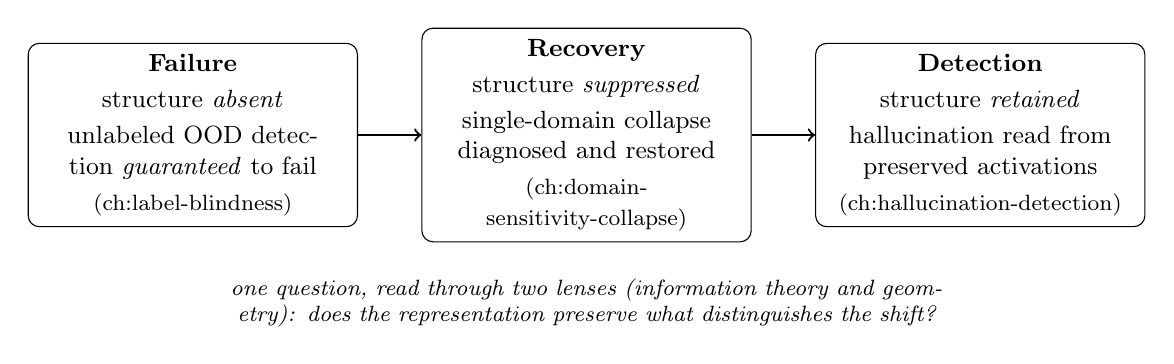
\begin{tikzpicture}[every node/.style={font=\small}]
    \tikzset{stage/.style={draw, rounded corners, text width=3.9cm, align=center,
      minimum height=2.2cm, inner sep=4pt}}
    \node[stage] (fail) at (0,0)
      {\textbf{Failure}\\[2pt] structure \emph{absent}\\[2pt]
       unlabeled OOD detection \emph{guaranteed} to fail\\[2pt]
       {\footnotesize(\Cref{ch:label-blindness})}};
    \node[stage] (rec) at (5,0)
      {\textbf{Recovery}\\[2pt] structure \emph{suppressed}\\[2pt]
       single-domain collapse diagnosed and restored\\[2pt]
       {\footnotesize(\Cref{ch:domain-sensitivity-collapse})}};
    \node[stage] (det) at (10,0)
      {\textbf{Detection}\\[2pt] structure \emph{retained}\\[2pt]
       hallucination read from preserved activations\\[2pt]
       {\footnotesize(\Cref{ch:hallucination-detection})}};
    \draw[->, thick] (fail) -- (rec);
    \draw[->, thick] (rec) -- (det);
    \node[font=\footnotesize\itshape, text width=11cm, align=center, anchor=north]
      at (5,-1.7)
      {one question, read through two lenses (information theory and geometry):
       does the representation preserve what distinguishes the shift?};
  \end{tikzpicture}%
  }
  \caption[The dissertation's spine]{The dissertation's spine. A single
  condition, whether the learned representation preserves the structure that
  distinguishes a shift, governs three reliability settings along one arc.}
  \label{fig:intro-spine}
\end{figure}

\section{Problem Statement and Motivation}
\label{sec:intro:problem}

Detection begins with the representation, not the scoring rule. Once a model has
been trained, a downstream detector can use only the distinctions preserved in
the model's features. The first question is therefore not which detector to
apply, but whether the training objective retained the information that detector
would need. The three studies examine different answers to this question.

\paragraph{Unlabeled OOD detection: structure absent.}
A self-supervised or unsupervised objective does not directly optimize for the
label distinction that defines an OOD task. When the features selected by that
objective are independent of the label-relevant features, the resulting
representation contains no usable signal about whether an example is
in-distribution or out-of-distribution. Under this condition, changing the
downstream detector cannot solve the problem. \Cref{ch:label-blindness}
formalizes this failure as label blindness. Its Adjacent OOD benchmark targets
the high-overlap regime in which the failure is most pronounced.

\paragraph{Single-domain OOD detection: structure suppressed.}
Supervised training preserves the features needed to separate known classes, but
training on a single domain can reduce sensitivity to directions that distinguish
one domain from another. \Cref{ch:domain-sensitivity-collapse} identifies this
effect as Domain-Sensitivity Collapse and shows how it weakens distance-based and
logit-based OOD detectors. Unlike label blindness, this is a diagnosis rather
than an impossibility result: the shift-sensitive structure can be strengthened.
Teacher-Guided Training restores that sensitivity by distilling knowledge from a
frozen multi-domain teacher without changing the model's inference-time cost.

\paragraph{Hallucination in large language models: structure retained.}
A language model's intermediate activations may preserve information about an
unsupported generation even when the final output does not reveal the failure.
\Cref{ch:hallucination-detection} asks whether the dependence between activations
at different layers provides enough signal for detection. It develops a
contrastive probe over cross-layer activation pairs to read out that signal from
a frozen model. Here the problem is not to recover information lost during
training, but to identify and use information that remains available internally.

\section{Research Objectives and Contributions}
\label{sec:intro:contributions}

This dissertation asks two related questions: when does a model's representation
make failure detection possible, and what can be done when the necessary
information is missing or suppressed? The three studies answer these questions
in different settings, while the fourth contribution brings their conclusions
into a common framework.

\begin{enumerate}
  \item \textbf{A limit on unlabeled OOD detection.}
  \Cref{ch:label-blindness} establishes a condition under which unlabeled OOD
  detection must fail. When a self-supervised objective selects features that
  are independent of the label-relevant distinction, the resulting
  representation provides no signal with which a downstream detector can
  distinguish in-distribution from out-of-distribution examples. We
  call this failure mode label blindness. The chapter presents the
  Adjacent OOD benchmark, which targets the high-overlap regime in which this
  limitation is most apparent. Full proofs appear in \Cref{app:proofs}.

  \item \textbf{A diagnosis and remedy for single-domain OOD detection.}
  \Cref{ch:domain-sensitivity-collapse} identifies Domain-Sensitivity Collapse
  (DSC), a process by which single-domain supervised training reduces variation
  along feature directions that distance- and logit-based detectors need. The
  resulting bounds diagnose why these detectors lose sensitivity without
  claiming that detection is impossible. The chapter then introduces
  Teacher-Guided Training (TGT), a training-time objective that distills a
  frozen multi-domain teacher to strengthen the suppressed directions without
  adding inference-time cost. Proofs appear in \Cref{app:dsc-proofs}.

  \item \textbf{A detector based on cross-layer language-model activations.}
  \Cref{ch:hallucination-detection} examines whether a language model retains
  information about hallucination in the dependence between its intermediate
  activations. A feasibility-by-trainability argument motivates a one-class
  contrastive probe over cross-layer activation pairs. The resulting detector
  matches or, in the mean, outperforms the strongest engineered probe in the
  comparison. An ablation also confirms a falsifiable prediction of the argument:
  symmetric contrastive supervision should fail. Proofs appear in
  \Cref{app:mi-hallucination-proofs}.

  \item \textbf{A common framework for detectability.}
  Taken together, the studies organize these problems around a single
  condition: whether the model's representation preserves the information
  needed to distinguish failure from ordinary behavior. Information theory
  describes whether that information remains, while feature-space geometry
  describes how it is organized and whether a detector can use it. Across the
  three studies, the relevant information is absent, suppressed but
  recoverable, or retained and available for readout.
\end{enumerate}

\section{Methodology and Approach}
\label{sec:intro:methodology}

The dissertation combines theoretical analysis with empirical evaluation. Each
study begins with the same object---a trained model's representation---and asks
what information it preserves about the distinction a detector must make.
\Cref{ch:background} develops the two perspectives used to answer that question:
information theory and feature-space geometry
\citep{shannon1948mathematical,cover1999elements,tishby2000information}.

The information-theoretic analysis treats a representation as a channel between
an input and the distinction of interest. In \Cref{ch:label-blindness}, this view
is used to determine when an unlabeled learning objective yields a representation
with no information needed for OOD detection. The resulting proof identifies a
specific condition under which no detector built on that representation can
distinguish in-distribution from out-of-distribution examples.
In \Cref{ch:hallucination-detection}, the same perspective is used in the opposite
direction: dependence between cross-layer activations provides a basis for asking
whether information about generation quality remains available for detection.

The geometric analysis in \Cref{ch:domain-sensitivity-collapse} asks how the
surviving information is arranged in feature space. In particular, it measures
whether single-domain training reduces variation along the directions that
distance- and logit-based OOD detectors use. The theoretical bounds describe
this loss of sensitivity, while Teacher-Guided Training tests whether guidance
from a multi-domain teacher can restore the affected geometry.

Empirical evaluations test each analysis in its corresponding regime:
high-overlap OOD detection, single-domain shift detection, and activation-based
hallucination detection. Controlled comparisons and ablations evaluate the
predicted mechanisms in each regime.

These methods support different conclusions: a conditional impossibility result
for label blindness, a diagnosis and empirically tested remedy for
Domain-Sensitivity Collapse, and a feasibility argument supported by parity with
the strongest engineered hallucination probe.

\section{Dissertation Organization}
\label{sec:intro:organization}

The dissertation proceeds from shared foundations to three studies and then to a
joint conclusion. Following this introduction, \Cref{ch:background} develops the
information-theoretic and geometric concepts used throughout the dissertation.
\Cref{ch:literature-review} then situates the research within prior work on OOD
detection, representation learning, and hallucination detection.

The next three chapters present the main studies. \Cref{ch:label-blindness}
establishes the label-blindness result and introduces the Adjacent OOD benchmark.
\Cref{ch:domain-sensitivity-collapse} analyzes Domain-Sensitivity Collapse and
develops Teacher-Guided Training as a remedy. \Cref{ch:hallucination-detection}
turns to language models and develops a contrastive detector based on cross-layer
activations. \Cref{ch:conclusion} brings the findings together, discusses the
limits of the common framework, and identifies directions for further research.

The complete proofs are collected in three appendices. \Cref{app:proofs}
supports the label-blindness result, \Cref{app:dsc-proofs} contains the
Domain-Sensitivity Collapse analysis, and \Cref{app:mi-hallucination-proofs}
provides the theory for hallucination detection.

\section{Significance}
\label{sec:intro:significance}

The central significance of this dissertation is that it separates detector
failure from representation failure. A benchmark can show that a particular
detector performs poorly, but it cannot determine whether another scoring rule
could succeed on the same representation. The label-blindness result answers
that deeper question under a stated independence condition: if the learning
objective preserves no information about the relevant distinction, changing the
downstream detector cannot help.

This distinction also determines what kind of intervention is appropriate. When
the information is absent, the representation or its training objective must
change. When it has been suppressed, as in Domain-Sensitivity Collapse, training
can restore the affected directions; Teacher-Guided Training does so without
adding inference-time cost. When the information remains internally available,
as the hallucination study investigates, a detector can be designed to read it
out from activations the model already computes.

The Adjacent OOD benchmark exposes a high-overlap regime that broad benchmarks
can obscure. Teacher-Guided Training addresses representation collapse in
narrow-domain models, while activation-based hallucination detection provides a
single-pass alternative to repeated sampling. Together, the studies establish
both limits on detection and interventions for cases in which useful information
can be restored or read out.

% chapters/02_background.tex
% Drafted 2026-06-07. Readability pass 2026-07-21: connective prose and formal
% definitions re-authored for sequential explanation. Public labels and downstream
% notation are preserved; the mutual-information chain rule and information-
% bottleneck optimization direction are corrected.
% Shared formal vocabulary, per outlines/02_background.md.
% Two boundaries: (i) primitives-only — named phenomena/methods are defined where
% contributed (Label-Blindness=Ch.4, DSC/TGT=Ch.5, layer-pair probe=Ch.6), so v1's
% "Domain Feature Collapse" definition is deleted here and replaced by a DSC
% forward-pointer; (ii) Ch.2 DEFINES the primitive, Ch.3 surveys its use. Sections
% run tasks (2.1-2.5, ported from v1 §2) then the two lenses (2.6-2.8) in the order
% Ch.3 opens with them. Notation follows math_commands.tex; geometry matches Ch.5,
% the InfoNCE/DPI primitives match Appendix C. Citations are sparse by design.
\chapter{Background and Definitions}
\label{ch:background}

This chapter defines the concepts used by more than one results chapter. The first
five sections specify the tasks and modeling settings. The final three introduce
information theory and representation geometry. Named results and methods remain
in the chapters that contribute them
(\Cref{ch:label-blindness,ch:domain-sensitivity-collapse,ch:hallucination-detection}).
\Cref{ch:literature-review} reviews how prior work uses the same concepts. Citations
here are therefore limited to foundational attributions.

\section{Out-of-Distribution Detection}
\label{sec:bg:ood}

Out-of-distribution (OOD) detection asks whether an input belongs outside the
model's training distribution. This dissertation focuses on \emph{semantic
shift}~\citep{yang2021generalized}. A semantic shift occurs when the true label is
not among the in-distribution labels, even if the input resembles the training
data.

\begin{definition}[Out-of-Distribution Detection]
Given an input $\rvx$ and a set of in-distribution labels $\sY_{\text{in}}$, OOD
detection determines whether the true label $\rvy$ lies outside that set:
\[
  \rvy \notin \sY_{\text{in}}.
\]
Equivalently, a probabilistic detector estimates
$P(\rvy \notin \sY_{\text{in}} \mid \rvx)$.
\label{def:bg:ood}
\end{definition}

The canonical baseline reads a confidence signal directly off a trained
classifier's output distribution.

\begin{method}[Maximum Softmax Probability (MSP)]
Given an input $\rvx$, the MSP method defines its OOD score as
$1-\mathrm{MSP}(\rvx)$, where
$\mathrm{MSP}(\rvx) = \max_{y \in \sY_{\text{in}}} P(y \mid \rvx)$~\citep{hendrycks2016baseline}.
\label{method:bg:msp}
\end{method}

We assume that a labeling function $f_{\rvy}$ assigns labels from the input alone.
Let $\sY_{\text{all}}$ contain every label that this function can produce over the
full input space. A training set need not contain them all, so in general
$\sY_{\text{in}} \subsetneq \sY_{\text{all}}$.

OOD methods differ in how they interact with training. A
\emph{training-agnostic} method, such as MSP, scores an existing classifier without
changing it. A \emph{training-aware} method changes the architecture, objective, or
augmentation procedure to improve detection.

OOD detection primarily addresses \emph{epistemic} uncertainty caused by limited
knowledge. It is distinct from \emph{aleatoric} uncertainty caused by irreducible
noise in the data. \Cref{ch:label-blindness,ch:domain-sensitivity-collapse} use
this OOD setting.

\section{Anomaly Detection}
\label{sec:bg:anomaly}

Anomaly detection and OOD detection both reject unusual inputs, but they use
different notions of unusual. \Cref{tab:bg:anomaly-ood} summarizes the distinction.

\begin{table}[H]
  \centering
  \caption{Typical distinctions between anomaly detection and OOD detection.}
  \label{tab:bg:anomaly-ood}
  \begin{tabular}{@{}lll@{}}
    \toprule
    & \textbf{Anomaly detection} & \textbf{OOD detection} \\
    \midrule
    Target
      & \shortstack[l]{Atypical points within\\a modeled domain}
      & \shortstack[l]{Inputs outside the modeled\\label set or distribution} \\
    Training data
      & \shortstack[l]{Usually normal examples\\from one class}
      & \shortstack[l]{Usually examples from several\\in-distribution classes} \\
    Evaluation
      & \shortstack[l]{Separates normal points\\from rare deviations}
      & \shortstack[l]{Separates in-distribution from\\out-of-distribution inputs} \\
    \bottomrule
  \end{tabular}
\end{table}

Anomaly detection is therefore often a \emph{one-class} problem: training provides
normal examples but no examples of the anomalies that must later be rejected. The
same training pattern appears in the unlabeled detectors of
\Cref{ch:label-blindness}. The hallucination probe of
\Cref{ch:hallucination-detection} uses a related but supervised asymmetric
construction. Its training data contain both faithful and hallucinated
generations, but only faithful generations form a mutual-positive class;
hallucinated generations otherwise act as negatives while retaining their own
cross-layer view pairs as positives.

\section{Unlabeled Out-of-Distribution Detection}
\label{sec:bg:unlabeled}

Most OOD detectors are trained on labeled in-distribution data and repurpose a
supervised classifier's outputs, softmax confidence or logits, as the detection
signal. Not all do. We call a detector \emph{unlabeled} when its training uses only
the inputs and never the labels.

\begin{definition}[Unlabeled OOD Detection]
Let the in-distribution dataset be
\[
  \sD_{\text{in}}=\{(\rvx_i,\rvy_i)\}_{i=1}^{N}.
\]
An OOD detector is \emph{unlabeled} if training uses only the inputs. It produces
\[
  f_{\text{OOD}}\gets\mathrm{Train}(\{\rvx_i\}_{i=1}^{N})
\]
with no dependence on the labels $\{\rvy_i\}$.
\label{def:bg:unlabeled}
\end{definition}

Unlabeled detectors commonly use density estimation, reconstruction error, or
self-supervised representations. A pretrained model used without fine-tuning also
fits the definition because it never trains on the in-distribution labels.

These methods are useful when labels are expensive or when detection should not
depend on one classification task. They still estimate the same event as a labeled
detector, $P(f_{\rvy}(\rvx) \notin \sY_{\text{in}})$. \Cref{ch:label-blindness}
studies the limit created by removing labels from training.

\section{Dataset Domain and the Single-Domain Setting}
\label{sec:bg:domain}

A \emph{domain} records the conditions under which data are produced, such as the
environment, sensor, or acquisition process. A domain-labeling function
$f_{\rvd}$ assigns each input a domain label,
$\rvd = f_{\rvd}(\rvx)$.

In the single-domain setting, every training input shares one domain $\rvd_1$:
\[
  f_{\rvd}(\rvx) = \rvd_1
  \qquad \text{for every in-distribution } \rvx.
\]
An input for which $f_{\rvd}(\rvx) \neq \rvd_1$ comes from a different domain.

For analysis, write the input as $\rvx=(\rvx_{\rvd},\rvx_{\rvy})$. The domain
features $\rvx_{\rvd}$ identify the generating conditions, while the class features
$\rvx_{\rvy}$ identify the target class. We assume that these feature sets are
independent within the training distribution:
\[
  I(\rvx_{\rvd};\rvx_{\rvy})=0.
\]
This independence is a modeling assumption, not a claim about the full input
space. Outside the training distribution, domain cues may also carry class
information.

\begin{definition}[Single-Domain Dataset]
A dataset is \emph{single-domain} with respect to $f_{\rvd}$ if every training
input has the same domain label $\rvd_1$. A multi-domain dataset contains training
inputs with more than one domain label. For the single-domain analyses in this
dissertation, the input admits domain and class features
$(\rvx_{\rvd},\rvx_{\rvy})$ that satisfy
$I(\rvx_{\rvd};\rvx_{\rvy})=0$ within the training distribution.
\label{def:bg:singledomain}
\end{definition}

Because the training domain is constant, class supervision does not directly
reward sensitivity to domain variation. \Cref{ch:domain-sensitivity-collapse}
studies how this setting can suppress domain-sensitive directions and how training
can restore them. \Cref{sec:bg:geometry} defines the geometric vocabulary used in
that analysis.

\section{Large Language Models and Hallucination}
\label{sec:bg:llm}

The hallucination study uses autoregressive language models and their intermediate
activations. This section defines both objects before introducing the
information-theoretic tools used to analyze them.

\begin{definition}[Large Language Model]
A \emph{large language model} (LLM) is a parameterized distribution over token
sequences. Let $\mathcal{X}$ be a finite vocabulary and $\mathcal{X}^{*}$ the set
of finite sequences over it. For a sequence
$\vx=(x_1,\ldots,x_T)$, an autoregressive model factorizes
\[
  \Pr_{\vtheta}(\vx)
  = \prod_{t=1}^{T}\Pr_{\vtheta}(x_t\mid x_{<t}),
  \qquad x_{<t}=(x_1,\ldots,x_{t-1}).
\]
The distribution is represented by a deep network, typically a Transformer. It is
trained on a corpus $\mathcal{D}$ by minimizing next-token cross-entropy:
\[
  \E_{\vx\sim\mathcal{D}}
  \left[-\sum_t\log\Pr_{\vtheta}(x_t\mid x_{<t})\right].
\]
\label{def:bg:llm}
\end{definition}

The term ``large'' refers to model and dataset scale rather than a fixed numerical
threshold. The analysis below depends on the autoregressive structure and exposed
activations, not on a particular parameter count.

\begin{definition}[Hallucination]
Let $\vx$ be a prompt and $\vy$ a continuation produced by the model. Fix a
reference world model $\mathcal{W}$ that represents the facts and sources
available for evaluation. A \emph{hallucination} occurs when a span
$\vy'\subseteq\vy$ presents as fact content that contradicts $\mathcal{W}$ or
cannot be verified from it.
\label{def:bg:hallucination}
\end{definition}

An \emph{extrinsic} hallucination conflicts with or lacks support from the external
world model $\mathcal{W}$. An \emph{intrinsic} hallucination is inconsistent with
the prompt or with earlier tokens in the generation. Because grounding is relative
to $\mathcal{W}$, an evaluation must state which facts and sources it treats as
authoritative.

\Cref{ch:hallucination-detection} does not assign its benchmark regime to either
category. It uses an operational label: a greedy generation is labeled
hallucinated when the benchmark's gold-reference evaluator marks it incorrect.
This convention fixes the detection target consistently without claiming that
every generation marked incorrect belongs to one hallucination taxonomy.

\paragraph{The residual stream.}
A Transformer maintains a hidden state at every token position and layer. For one
position, write the sequence as $h_1,\ldots,h_L$, where
$h_\ell\in\R^d$ is the state produced by layer $\ell$. This sequence is the
\emph{residual stream}.

The activations are available from one forward pass and require no resampling. An
internal-state detector can therefore score them directly.
\Cref{ch:hallucination-detection} learns from pairs of layers. The next two
sections define the information-theoretic tools that justify this pairing.

\section{Information Theory}
\label{sec:bg:infotheory}

Information theory~\citep{shannon1948mathematical} quantifies uncertainty and
statistical dependence. In this dissertation, it measures how much information a
representation retains about a target.

\begin{definition}[Entropy and Conditional Entropy]
The \emph{entropy} $H(\rvx)$ of a random variable $\rvx$ with distribution
$p(\vx)$ is its expected uncertainty. For discrete variables,
\[
  H(\rvx)=-\sum_{\vx}p(\vx)\log p(\vx).
\]
The \emph{conditional entropy} is the uncertainty remaining in $\rvy$ after
$\rvx$ is known:
\[
  H(\rvy\mid\rvx)
  =-\sum_{\vx,\vy}p(\vx,\vy)\log p(\vy\mid\vx).
\]
The corresponding definitions for continuous variables replace sums with
integrals. Entropy and conditional entropy satisfy the chain rule
\[
  H(\rvx,\rvy)=H(\rvx)+H(\rvy\mid\rvx).
\]
\label{def:bg:entropy}
\end{definition}

\begin{definition}[Mutual Information]
The \emph{mutual information} $I(\rvx;\rvy)$ is the reduction in uncertainty about
one variable after observing the other. Equivalently, it is the divergence between
the joint distribution and the product of the marginals:
\[
  I(\rvx;\rvy)
  =D_{\mathrm{KL}}\!\left(p(\vx,\vy)\,\middle\|\,p(\vx)p(\vy)\right).
\]
Here the Kullback--Leibler divergence is
\[
  D_{\mathrm{KL}}(p\|q)
  =\E_{\vx\sim p}\!\left[\log\frac{p(\vx)}{q(\vx)}\right].
\]
Mutual information is non-negative and equals zero exactly when the variables are
independent. Its chain rule is
\[
  I(\rvx;\rvy,\rvz)
  =I(\rvx;\rvz)+I(\rvx;\rvy\mid\rvz).
\]
\label{def:bg:mi}
\end{definition}

Processing cannot increase the information one variable contains about another.
The data processing inequality states this constraint.

\begin{definition}[Data Processing Inequality]
Suppose three random variables form a Markov chain
$\rvx\rightarrow\rvy\rightarrow\rvz$. Then $\rvz$ depends on $\rvx$ only through
$\rvy$, and
\[
  I(\rvx;\rvz)\le I(\rvx;\rvy).
\]
No transformation of $\rvy$ can increase its information about $\rvx$.
\label{def:bg:dpi}
\end{definition}

The inequality also applies when each of two variables is mapped to a learned
embedding. If $g_a$ and $g_b$ encode two layer activations, then
\[
  I(g_a(h_a);g_b(h_b))\le I(h_a;h_b).
\]
A positive lower bound at the embedding level therefore certifies positive
dependence between the underlying activations. \Cref{ch:hallucination-detection}
uses this fact, and \Cref{app:mi-hallucination-proofs} gives the formal statement.

\section{Sufficiency, Information Bottleneck, and InfoNCE}
\label{sec:bg:ib}

Three concepts turn the information-theoretic view into a tool for representation
learning. Sufficiency states what a representation must retain. The information
bottleneck adds a compression objective. InfoNCE supplies a contrastive lower bound
that can be estimated from samples.

\begin{definition}[Minimal Sufficient Statistic]
A statistic $T(\rvx)$ is \emph{sufficient} for $\rvy$ if it retains all the
information that $\rvx$ carries about $\rvy$:
\[
  I(\rvx;\rvy\mid T(\rvx))=0.
\]
It is \emph{minimal} if it is a function of every other sufficient statistic. A
minimal sufficient statistic is therefore the most compact representation that
loses no information about $\rvy$.
\label{def:bg:mss}
\end{definition}

\begin{definition}[Information Bottleneck]
Given an input $\rvx$ and target $\rvy$, the \emph{information
bottleneck}~\citep{tishby2000information} seeks a representation $\rvz$ that
retains target information while compressing the input. One minimization form is
\[
  \min_{p(\vz\mid\vx)}\;
  \mathcal{L}_{\mathrm{IB}}
  = I(\rvz;\rvx)-\beta I(\rvz;\rvy),
\]
where $\beta>0$ controls the tradeoff between compression and target retention.
Under appropriate capacity and optimization assumptions, this objective favors a
minimal sufficient representation of the target.
\label{def:bg:ib}
\end{definition}

Sufficiency drives the result of \Cref{ch:label-blindness}. If the surrogate task
is independent of the class-relevant features, its minimal sufficient
representation contains no class information. A detector built only on that
representation cannot distinguish the held-out classes.

The language-model analysis asks a different question: whether information remains
between two layer representations. Because this quantity must be estimated from
samples, the analysis uses a contrastive lower bound.

\begin{method}[InfoNCE Lower Bound]
Under the standard InfoNCE sampling construction, let two encoded views
$\mathrm{view}_a$ and $\mathrm{view}_b$ be scored against $K-1$ negatives. If
$\mathcal{L}_{\mathrm{NCE}}$ is the resulting loss~\citep{oord2018representation},
then
\[
  I(\mathrm{view}_a;\mathrm{view}_b)
  \ge \log K-\mathcal{L}_{\mathrm{NCE}}.
\]
Thus $\mathcal{L}_{\mathrm{NCE}}<\log K$ gives a strictly positive lower bound on
the mutual information between the views.
\label{method:bg:infonce}
\end{method}

InfoNCE underlies modern contrastive representation learning. Self-supervised
methods apply it to augmented views~\citep{chen2020simclr}. Supervised contrastive
learning instead treats examples from the same class as
positives~\citep{khosla2020supervised}.

\Cref{ch:hallucination-detection} starts from this construction but uses an
asymmetric supervised contrastive objective: faithful samples form a
mutual-positive class, whereas each hallucinated sample retains only its own
cross-layer views as positives. Because this is a multi-positive supervised
specialization, the standard $\log K$ threshold above does not transfer unchanged.
The class-conditioned bound for the chapter's exact objective appears in
\Cref{app:mi-hallucination-proofs}.

\section{Representation Geometry}
\label{sec:bg:geometry}

Representation geometry asks how learned features are arranged in space. Of
particular interest is how variance is distributed across feature directions.

Let $z=f_\theta(\rvx)\in\R^d$ be the feature assigned to an input from a
$C$-class dataset. Let $\Sigma$ be the empirical covariance of these features,
with eigenvalues $\lambda_1\ge\cdots\ge\lambda_d$. The covariance decomposes as
\[
  \Sigma=\Sigma_{\mathrm{between}}+\Sigma_{\mathrm{within}}.
\]
The between-class component has rank at most $C-1$. If training drives
$\Sigma_{\mathrm{within}}$ toward zero, the representation concentrates its
variance in at most $C-1$ directions.

\begin{definition}[Anisotropy: Participation Ratio and Effective Rank]
The \emph{participation ratio} and \emph{effective rank} measure the concentration
of a covariance spectrum:
\[
  \mathrm{PR}(\Sigma)
  =\frac{(\sum_i\lambda_i)^2}{\sum_i\lambda_i^2},
  \qquad
  r_{\mathrm{eff}}(\Sigma)
  =\exp\!\left(-\sum_i\hat{\lambda}_i\log\hat{\lambda}_i\right),
\]
where $\hat{\lambda}_i=\lambda_i/\sum_j\lambda_j$. Both quantities estimate how
many directions carry meaningful variance. A representation with
$r_{\mathrm{eff}}\ll d$ is strongly anisotropic.
\label{def:bg:anisotropy}
\end{definition}

\begin{definition}[Class-Discriminative Subspace]
Let $v_1,\ldots,v_k$ be the top eigenvectors of $\Sigma$. In the supervised
settings studied here, these directions capture the dominant between-class
variation. We therefore write the \emph{class-discriminative subspace} as
\[
  \mathcal{S}_{\mathrm{cls}}
  =\operatorname{span}\{v_1,\ldots,v_k\}.
\]
Let $P$ be the orthogonal projector onto $\mathcal{S}_{\mathrm{cls}}$ and let
$P_\perp=I-P$. Every feature decomposes as
\[
  z=z_\parallel+z_\perp,
  \qquad z_\parallel=Pz,
  \qquad z_\perp=P_\perp z.
\]
The term ``class-discriminative'' records the supervised alignment assumption. If
that alignment does not hold, the same construction is simply the dominant
principal subspace. A domain shift with little in-distribution variance may appear
primarily in the complementary directions $z_\perp$.
\label{def:bg:clssubspace}
\end{definition}

Detection scores respond differently to this geometry. Euclidean
nearest-neighbor scores~\citep{sun2022out} are often dominated by high-variance
directions. A regularized Mahalanobis score~\citep{lee2018simple} can amplify a
low-variance direction only if the representation preserves useful separation
there.

Logit-based scores read features through the classifier head. Maximum softmax
probability (\Cref{method:bg:msp}) and the energy score~\citep{liu2020energy}
cannot respond to a direction that lies in the head's null space.
\Cref{ch:domain-sensitivity-collapse} makes these conditions precise. Neural
collapse describes the limiting geometry that motivates the analysis.

\begin{definition}[Neural Collapse]
\emph{Neural collapse}~\citep{Papyan2020nc} is a terminal-phase classification
geometry. Within-class variance vanishes,
$\Sigma_{\mathrm{within}}\to0$, and the class means form a
$(C-1)$-simplex equiangular tight frame. The remaining $d-(C-1)$ directions carry
zero variance in the limiting representation.
\label{def:bg:neuralcollapse}
\end{definition}

Neural collapse is an asymptotic limit. When shift-sensitive directions lie in the
collapsed complement, a detector cannot use them through the learned
representation. \Cref{ch:domain-sensitivity-collapse} studies the corresponding
finite-training geometry and a remedy. The formal results appear in
\Cref{app:dsc-proofs}.

The chapter has now defined the two analytical perspectives used in the
dissertation. \Cref{ch:literature-review} reviews their use in prior work, and the
three results chapters apply them to their respective detection problems.

% chapters/03_literature_review.tex — stub. Carry-over from v1 §3.
% See ../outlines/00_dissertation_outline.md (Chapter 3).
\chapter{Literature Review}
\label{ch:literature-review}

TODO: port and update from v1 §3 (Information Theory in ML; Representation
Learning; OOD Detection; Hallucination Detection; Model Architectures).

% chapters/04_label_blindness.tex — stub.
% Integrates the ICLR 2025 paper "Can We Ignore Labels in OOD Detection?".
\chapter{Label Blindness in Unlabeled OOD Detection}
\label{ch:label-blindness}

TODO: label blindness theorem, Adjacent OOD benchmark, experiments.

% chapters/05_domain_feature_collapse.tex — BLANK, pending source paper.
% A NEW paper replaces the prior AAAI submission; do NOT port v1 §5.
% Drop the new source into ../sources/<slug>/ and see
% ../outlines/00_dissertation_outline.md (Chapter 5) before drafting.
\chapter{Domain Feature Collapse in Single-Domain OOD Detection}
\label{ch:domain-feature-collapse}

TODO: awaiting replacement source paper. Intentionally left blank.

% chapters/06_hallucination_detection.tex — BLANK, pending source paper.
% The MI-Hallucination paper will be provided; do NOT port v1 §6 (a proposal,
% not results). See ../outlines/00_dissertation_outline.md (Chapter 6).
\chapter{Information-Theoretic Hallucination Detection}
\label{ch:hallucination-detection}

TODO: awaiting MI-Hallucination source paper. Intentionally left blank.

% chapters/07_conclusion.tex
% Rewritten 2026-07-21 from a claim-and-scope matrix for Chapters 4--6.
% Objective: conclusion-level synthesis rather than another chapter recap. The
% three studies are treated as distinct evidential cases, not points on a common
% quantitative scale. Information theory describes dependence; geometry describes
% organization and accessibility. They are complementary, not interchangeable.
% Framing locks: guaranteed failure is Ch.4-only; Ch.5 is diagnostic and recoverable;
% Ch.6 claims parity, reports the Natural Questions losses, and never claims SOTA.
% No new results, re-derivations, or hard-coded result values appear here.
\chapter{Conclusion}
\label{ch:conclusion}

A reliability detector can fail for two different reasons. Its scoring rule may
be too weak to extract a distinction that the model represents, or the model may
not represent that distinction in the first place. These cases call for different
responses. A better readout can address the first. The second requires a change to
the learned features or the objective used to train them. The detector may instead
need access to additional information. This dissertation has separated those cases
across two forms of out-of-distribution (OOD) detection and one form of
hallucination detection.

Information theory and representation geometry made that separation possible.
Information theory asks whether the representation remains statistically dependent
on the target decision. Geometry describes how relevant variation is arranged
across feature directions and whether a particular detector can use it.
The two perspectives address the same representational question without measuring
an identical object. The three studies likewise form a conceptual progression,
not a shared numerical scale: \Cref{ch:label-blindness} establishes a conditional
failure boundary, \Cref{ch:domain-sensitivity-collapse} diagnoses and repairs
suppressed sensitivity, and \Cref{ch:hallucination-detection} constructs a detector
for a signal that remains accessible inside a frozen model. This chapter states
what those results jointly establish, where the common framework stops, and which
questions follow from it.

\section{What the Dissertation Establishes}
\label{sec:concl:summary}

Each study supplies a different kind of evidence. The first proves a limit under a
stated independence condition. The second gives conditional bounds and tests a
training-time remedy. The third uses a feasibility argument to motivate a detector
and evaluates the resulting construction. Their conclusions should therefore be
combined without treating their guarantees as interchangeable.

\subsection{A Conditional Limit on Unlabeled OOD Detection}

\Cref{ch:label-blindness} asks whether OOD detection can use features produced
without the labels that define the eventual task. When the self-supervised or
unsupervised surrogate task is independent of the label-relevant features, the
minimal sufficient representation for that task contains no
information about the required label distinction. A detector restricted to that
representation then has no statistic from which to recover the distinction. The
Label Blindness Theorem makes this a \emph{guaranteed-failure} result under its
independence condition (\Cref{mainbodyfailood}). It is not a claim that every
unlabeled representation fails, nor that strong performance on conventional OOD
benchmarks is impossible.

The Adjacent OOD benchmark makes the condition empirically visible. Many benchmark
pairs differ through dataset-level cues that an unlabeled representation can use
without encoding the held-out class distinction. Adjacent OOD increases the overlap
between in-distribution and OOD inputs so that incidental cues provide less help.
High overlap does not by itself imply label blindness; the independence condition
remains essential. The benchmark instead tests the setting in which dependence on
the relevant label features matters most. Together, the theorem and benchmark
distinguish success on a chosen dataset pair from a general guarantee that an
unlabeled objective will preserve whatever a future OOD task requires.

\subsection{A Geometric Diagnosis and Training-Time Recovery}

\Cref{ch:domain-sensitivity-collapse} studies a different failure. Here labels are
available, but single-domain supervision rewards separation among the known classes
without directly rewarding sensitivity to changes of domain. Domain-Sensitivity
Collapse (DSC) describes the resulting concentration of variance in a
class-discriminative subspace and the suppression of directions that would respond
to domain shift. Under the conditions developed in the chapter, distance-based and
logit-based OOD scores lose separation because both operate on the affected
features (\Cref{thm:dsc:dist-fail,prop:dsc:msp-insens}). These bounds diagnose a
mechanism. They do not prove that every single-domain model must fail or that no
intervention can recover the signal.

Teacher-Guided Training (TGT) tests the diagnosis by acting on the representation
rather than replacing the scorer. It transfers the class-suppressed residual of a
frozen multi-domain teacher into the student during training, after which the
teacher and auxiliary head are discarded (\Cref{sec:dsc:method}). The resulting
changes in feature geometry accompany improvements for the post-hoc scorers studied
in the chapter, with the most consistent gains in the distance-based family that
the DSC analysis directly addresses. TGT therefore supplies more than a second OOD
method: it shows that a geometric account of lost sensitivity can identify a
training-time intervention, while retaining ordinary student-only inference.

\subsection{Detection from Cross-Layer Language-Model Activations}

\Cref{ch:hallucination-detection} begins from a frozen language model, where
retraining the underlying representation is outside the detection setting. The
question is whether intermediate activations contain a usable distinction between
faithful and hallucinated generations. Dependence between layers makes a
contrastive objective over layer-pair views well-posed. The chapter uses this
feasibility argument to motivate Contrastive+Recon, a one-class contrastive probe
with an auxiliary reconstruction channel (\Cref{sec:hd:method}). Cross-layer
dependence alone does not establish that hallucination labels are recoverable.
Evidence comes from the detector's discrimination performance and the predicted
failure of symmetric supervision (\Cref{sec:hd:results,sec:hd:ablations}).

Across the main comparison, Contrastive+Recon occupies the same performance band
as the strongest engineered probe. It \emph{matches-or-outperforms, in the mean,}
that baseline. This is a parity claim rather than dominance. The method wins some
comparisons, ties others within the observed variation, and loses on Natural
Questions for both models. Its cross-dataset results also support parity under
transfer rather than a transfer win (\Cref{sec:hd:transfer}). These outcomes support the cross-layer design
rationale. They do not show that the probe is an optimal readout or that the
information-theoretic argument selects the best detector for every dataset.

\subsection{A Joint Finding About Representation and Detection}
\label{subsec:concl:synthesis}

The three studies answer one question under different constraints: does the model
representation available to the detector contain the distinction the detector must
make? \Cref{ch:label-blindness} studies a condition under which the answer is no.
\Cref{ch:domain-sensitivity-collapse} studies features whose domain sensitivity has
been suppressed by training and shows that the geometry can be changed.
\Cref{ch:hallucination-detection} studies a frozen model for which the relevant
signal remains accessible in intermediate activations. The failure, recovery, and
detection sequence names these cases. It does not rank the studies by a common
amount of information because the target and evidence differ across models.

What carries across them is a constraint on method design. Improving a scorer
cannot recover a distinction that is absent from every input the scorer receives.
When training has reduced sensitivity to a distinction, changing the representation
may be more effective than continuing to refine a post-hoc score. When the signal
remains available, the readout and its supervision determine how much of that signal
is usable in practice. Representation content is therefore a necessary part of a
detection analysis, but it is not sufficient by itself. Accessibility and
estimation still matter, as does detector capacity.

This distinction is the dissertation's common contribution. It changes the first
question asked about a failed detector. Instead of immediately selecting another
score, the analysis asks what distinction the score can observe and whether training
preserved it. The available evidence then determines whether to change the readout
or the representation. The three studies do not produce a universal detector. They
provide three ways to answer that prior question and demonstrate the different
interventions that follow from its answer.

\section{Implications of the Common Framework}
\label{sec:concl:implications}

The common framework matters beyond the individual methods because it separates
problems that are often combined under the broad label of detection failure. It
also clarifies what the two analytical perspectives contribute and how evaluation
can test a proposed mechanism.

\subsection{Representation Failure and Detector Failure}
\label{subsec:concl:representation}

An observed detection error does not reveal whether the representation or the
scoring rule caused it. Benchmarking several scores on fixed features can compare
readouts, but it cannot show that the features contain every distinction the task
requires. Label blindness supplies the clearest case: once the stated independence
condition removes the target distinction, no post-hoc score on that representation
can reconstruct it. DSC supplies a less absolute case in which existing features
respond weakly to domain shift and training can restore useful directions. The
hallucination study addresses the remaining case, where a single-pass readout can
extract a distinction from activations already computed by the model.

These cases suggest an intervention order. First determine what the detector can
observe. If the required signal is absent, the learning objective or representation
must change unless the detector receives new inputs. External retrieval and repeated
generations can change what is observable without retraining the base model. If the
signal has been suppressed but remains recoverable, a
training-time objective can strengthen it. If it is already available, readout
design becomes the relevant problem. This order is a practical diagnostic, not a
theorem that guarantees the chosen intervention will succeed.

\subsection{Information Theory and Geometry as Complementary Evidence}
\label{subsec:concl:lenses}

Information theory and representation geometry contribute different evidence to
this diagnostic. Mutual information states whether statistical dependence remains
between a representation and a target. It can establish an impossibility boundary
when that dependence vanishes, or justify an objective when a lower bound can be
optimized. It does not, by itself, show that a simple detector can recover the
dependence from finite data. Geometry describes where variation lies, how strongly
it is concentrated, and whether the directions used by a scorer respond to the
shift. A favorable geometric arrangement can make a signal accessible, but a
geometric statistic alone does not establish its relationship to every target.

The studies use the perspective suited to each claim. Label blindness and the
cross-layer probe are expressed through dependence and information bounds. DSC uses
feature spectra and subspaces, then relates them to scorer sensitivity. Similar training
processes may affect both information and geometry, but this dissertation does not
prove that mutual-information loss and rank collapse are equivalent. Its more
defensible methodological conclusion is that reliability analysis benefits from
both questions: whether target dependence remains and how the surviving variation
is organized for the detector that must use it.

\subsection{Evaluation as a Test of Mechanism}
\label{subsec:concl:eval}

The experiments also illustrate a role for evaluation beyond producing an aggregate
ranking. A theoretical or mechanistic claim should identify a regime in which its
predicted effect becomes visible. Adjacent OOD reduces incidental separation so
that label dependence becomes consequential. The single-domain experiments measure
feature rank alongside OOD performance and compare in-domain with out-of-domain
shifts, allowing the geometric diagnosis and the proposed recovery to be examined
together. In hallucination detection, compute-matched comparisons separate the
benefit of activation access from the cost of repeated sampling. The symmetric
supervision ablation and cross-dataset evaluation test predictions about the learned
signal rather than only its average score.

Negative and uneven results are informative under this view. The Natural Questions
losses identify a setting in which the cross-layer rationale does not match the
strongest engineered probe. Variable TGT gains identify where teacher--student
complementarity or scorer choice affects recovery. Strong performance by unlabeled
methods on far-OOD pairs shows why label blindness may be hidden rather than
disproving the conditional result. A benchmark supports a reliability claim only
to the extent that its design exposes the mechanism and scope named by that claim.

\section{Scope and Limitations}
\label{sec:concl:limitations}

The common framework does not amount to a universal necessary-and-sufficient theory
of detectability. It combines one conditional impossibility result, one conditional
geometric diagnosis with an empirical remedy, and one supported feasibility
argument. None establishes that representation quality alone determines detection
performance, and none identifies an optimal detector for every distribution.

\paragraph{Label blindness.}
The strict result assumes independence between the surrogate task and the
label-relevant features. Real self-supervised objectives often share some structure
with later semantic tasks, so the exact theorem describes a boundary rather than an
expected field failure rate. Approximate label blindness is correspondingly harder
to diagnose because small dependence may still be useful to a strong readout. The
Adjacent OOD construction examines substantial feature overlap, which makes the
failure easier to expose. It does not represent the full range of shifts encountered in
deployment. Overlap and independence must not be treated as the same condition.

\paragraph{Domain-Sensitivity Collapse.}
The DSC bounds apply under stated assumptions about feature anisotropy and dominant-
subspace matching, together with limits on scorer sensitivity. They explain when the
studied scores lose separation; they are not convergence results across every
single-domain training setting.
The empirical evaluation covers a varied but finite collection of domains and shows
that improvements differ across scorers and teacher--student pairings. TGT also
depends on the teacher containing domain-sensitive structure that the student lacks.
A teacher with limited coverage or a representation too similar to the student can
provide a weaker recovery signal.

\paragraph{Hallucination detection.}
Contrastive+Recon and the strongest engineered baseline occupy the same performance
band rather than separating consistently. The Natural Questions losses remain
unexplained, and the transfer results do not remove them. The feasibility argument
supports the use
of cross-layer views but does not prove that the selected layers or one-class
objective extract the available signal optimally. The same uncertainty applies to
the reconstruction channel and distance scorer. The evaluation is also limited to
the studied open-weights models and short-answer tasks. It requires white-box
activation access and uses operational labels produced by an automatic evaluator.
These constraints limit both applicability and the precision of the target being
learned (\Cref{sec:hd:limitations}).

\paragraph{The synthesis.}
The absent, suppressed, and accessible cases organize the contributions, but they
are not exhaustive states with fixed thresholds. A representation may preserve a
weak signal that is usable only with more data or a nonlinear readout. Additional
context may also be necessary. The detector can introduce information through
retrieval or sampling, and another external source can change the task again. The
framework should therefore separate sources of failure and select the next analysis;
it is not a complete scalar measure of reliability.

\section{Future Directions}
\label{sec:concl:future}

The limitations lead to research questions that test and extend the framework
rather than simply applying the existing methods to more benchmarks.

\paragraph{Measure label blindness by degree.}
A useful diagnostic would estimate how much dependence a particular learning
objective preserves about a proposed label distinction. Such a measure would need
to account for the data distribution as well as the objective and labels; the risk
cannot be inferred from the objective name alone. Estimation before or during
training could turn strict label blindness from a boundary result into a screening
tool, while experiments could determine how much residual dependence different
detectors require.

\paragraph{Relate information loss to geometric collapse under explicit
conditions.}
DSC was developed geometrically, while the other studies rely primarily on
information-theoretic arguments. Future work could identify assumptions under which
changes in target mutual information imply changes in the feature spectrum or in a
shift-sensitive subspace, and also construct counterexamples where they diverge.
This would test the relationship between the two perspectives without presuming
that they measure the same object. It could also provide diagnostics that connect a
geometric warning to the target dependence a deployment actually requires.

\paragraph{Recover domain sensitivity beyond a fixed teacher.}
TGT inherits both the strengths and the blind spots of its multi-domain teacher.
Future methods could compare teachers with different coverage and select residual
targets adaptively. Another approach would recover domain-sensitive variation
without a fixed teacher.
The unresolved in-domain OOD regime is especially important because class and domain
cues overlap there more strongly. Progress should be evaluated through changes in
the representation as well as changes in the final OOD score, so that an improved
number can be tied to the proposed recovery mechanism.

\paragraph{Generalize and act on the hallucination signal.}
The cross-layer construction should be tested across model families and scales,
including different generation formats, with particular attention to the Natural
Questions shortfall and to settings where activations are unavailable. Layer
selection remains open, as do the relative roles of contrastive and reconstruction
supervision. A further
step would move from detection to mitigation by asking whether the identified
directions can safely alter generation rather than merely flag it. That question
requires a causal evaluation of the intervention and cannot be answered by detector
performance alone.

\section{Concluding Remarks}
\label{sec:concl:remarks}

This dissertation began from a practical problem: models can remain confident when
their inputs or outputs fall outside what their training supports. Its central
conclusion is not that one detector solves this problem across domains. It is that
detector design should begin by establishing what distinction the available
representation contains. \Cref{ch:label-blindness} marks a condition under which
that distinction is absent. \Cref{ch:domain-sensitivity-collapse} shows that
training can restore suppressed sensitivity, while
\Cref{ch:hallucination-detection} demonstrates a readout for a signal retained
inside a frozen model.

The resulting framework separates limits from repairable failures and repairable
failures from readout problems. Information theory and geometry provide different
evidence for making those distinctions. Their joint value lies in directing the
analysis to the representation before another score is added on top.
When the representation keeps it, a detector can read it out.


%*******************************************
% APPENDICES  (one file per appendix, in appendices/)
%*******************************************
\begin{appendices}
% appendices/A_proofs.tex — stub. Fill from ../v1/AppendixA.tex.
\chapter{Theoretical Proofs for Label Blindness}
\label{app:proofs}

TODO: mathematical proofs for the Label Blindness Theorem.

% appendices/B_domain_feature_collapse_proofs.tex — BLANK, pending.
% Tied to Chapter 5's replacement paper; do NOT port v1/AppendixB.tex until the
% new paper's theory is fixed. See ../outlines/00_dissertation_outline.md.
\chapter{Theoretical Proofs for Domain Feature Collapse}
\label{app:domain-feature-collapse-proofs}

TODO: awaiting replacement source paper. Intentionally left blank.

\end{appendices}

%*******************************************
% BIBLIOGRAPHY
%*******************************************
\bibliographystyle{plainnat}
\bibliography{references}

\end{document}
